\documentclass{article}
\DeclareMathSizes{10}{10}{7}{7}
\usepackage{amsmath}
\usepackage{ amssymb }
\usepackage{tikz, graphicx}
\usepackage{geometry}
\usepackage[makeroom]{cancel}
\usepackage[export]{adjustbox}
\usepackage{upgreek}
\DeclareMathOperator{\sech}{sech}
\usepackage{subcaption}
\usepackage{hyperref}
\usepackage{caption}
\hypersetup{
    colorlinks=true,
    linkcolor=blue,
    filecolor=magenta,      
    urlcolor=blue,
    }
\usepackage{float}
\restylefloat{table}

\geometry{legalpaper, margin=0.7in}

\title{Splashing in the waves with the KdV equation}
\author{Liam Watson}
\begin{document}
\maketitle

\section{Intorduction}
We are tasked with investigating the behavior of the so called modified KdV equation.
\begin{align}
&u_t + u_{xxx} + u^2u_x = 0 \\
&u(L,t) = u(-L,t) \\
&u_x(L,t) = u_x(-L,t) \\
&u_{xx}(L,t) = u_{xx}(-L,t) \\
&u(x,0) = A \theta(\frac{1}{2}- |x|) 
\end{align}
with $\theta$ being Heavyside’s step function
\begin{align*}
\theta(x) &=
\begin{cases}
 1 & \text{if } x > 0 \\
 0 & \text{if } x \leq 0 \\
\end{cases}
\\
\theta(x) &=
\begin{cases}
 1 & \text{if } -\frac{1}{2} < x < \frac{1}{2} \\
 0 & \text{if } -\frac{1}{2} \leq x \geq \frac{1}{2}\\
\end{cases}
\end{align*}
The goals of this report are as follows:
\begin{enumerate}
\item Employ a numerical method for the equations solution 
\item Use influence functions to describe an analytical solution to the linearised equation
\item Investigate the asymptotic behavior of the KdV equation 
\item Compare the numerical and analytical results
\end{enumerate}
\section{Numerical solution}
For the numerical method we choose the sudospectral method as it exhibits better stability and performance properties. \\
Using the FD method is also a valid method and I will briefly include a derivation but not an implimentation. \\
The sudospectral method requires us to use a center difference for a the approximation of the time derivative. 
\begin{align*}
u_t = \frac{u_{j,k+1}-u{j,k-1}}{2\tau}
\end{align*}
For the spacial derivatives we expand using a fourier series as follows:
\begin{align*}
u_{xxx} = \sum_{n=\frac{-N}{2}}^{\frac{N}{2}-1}\left(\frac{2\pi i n}{L}\right)^3 \widehat{u_n}(t_k)e^{\frac{2\pi i n j}{N}}
\end{align*}
The nonlinear term is not quite as simple but we can after a little effort find a fourier series representation for it. Notice that:
\begin{align*}
u^2u_x = \frac{\partial}{\partial x}\left(\frac{u^3}{3}\right)
\end{align*}
We call the expression in the brackets $f(x,t)$ which we expand in a Fourier Series.
\begin{align*}
f(x,t) = \sum_{n=\frac{-N}{2}}^{\frac{N}{2}-1}\left(\frac{2\pi i n}{L}\right) \widehat{\left(\frac{u^3}{3}\right)}_n(t_k)e^{\frac{2\pi i n j}{N}}
\end{align*}
We now have expressions for all the terms in the modified KdV equation and can impliment a numerical solution. 
\section{Analytic solutions}
In this section we assume that $A$ is small $A^2\approx0.1$ and as such the nonlinearity should be neglidgable compared to the displersion and we can get a good approximate analytical solution by solving the linearized KdV equation with the same IC and BC's:
\begin{align*}
u_t + u_{xxx} = 0
\end{align*}
\subsection{Influence equation}
\begin{align*}
u(x,t) = \int U(k,t)e^{-ikx}dk
\end{align*}
Assume we can differentiate under the integral
\begin{align*}
&u_{xxx} = \int (-ik)^3U(k,t)e^{-ikx}dk \\
u_t = \int U_t(k,t)e^{-ikx}dk
\end{align*}
Putting these back into the linearized KdV equation
\begin{align*}
\int (U_t + ik^3 U) e^{-ikx}dk = 0
\end{align*}
We know the Fourier Transform of zero is zero so the integrad must be zero. The integrand is a simple ODE in time which we can easily solve:
\begin{align*}
U_t + ik^3U = 0 \implies U(k,t) = F(k)e^{ik^3t}
\end{align*}
Now that we know $U(k,t)$ we can put it into the expression we had for $u(x,t)$.
\begin{align*}
u(x,t) = \int F(k) e^{ik^3t}e^{-ikx}dk
\end{align*} 
Now we need to determine $F(k)$ using the IC and we find
\begin{align*}
F(k) &= \frac{1}{2\pi} \int_{\infty}^{\infty} f(x^\prime) e^{ikx^\prime}dx^\prime \\
&= \frac{A}{2\pi} \left[ \int_{-\infty}^\frac{-1}{2} 0e^{ikx^\prime}dx^\prime        \int_\frac{-1}{2}^\frac{1}{2}e^{ikx^\prime}dx^\prime \int^{\infty}_\frac{1}{2} 0e^{ikx^\prime}dx^\prime\right] \\
&= \frac{A}{2\pi}\int_{-\frac{1}{2}}^\frac{1}{2}e^{ikx^\prime}dx^\prime \\
&= \frac{A}{2\pi}\frac{2\sin(\frac{k}{2})}{k}
\end{align*}
We now need to use the Convolution theorem to determine the influence function. We notice that the integrand is close to the Airy function Fourier Transform $e^{\frac{ik^3}{3}}$. We can form an equation so satisfy both the convolution theorem and the Airy function
\begin{align*}
e^{ik^3t}e^{-ikx} &= e^{\frac{i(\frac{k}{\alpha})^3}{3}}e^{-ik(x-x^\prime} \\
ik^3 &= \frac{ik^3}{\alpha^3 t} \\
\alpha &= \frac{1}{3\sqrt[3]{t}}
\end{align*}
Hence we find the influence function to be
\begin{align*}
G(x,t;x^\prime, 0) = \frac{1}{3\sqrt[3]{t}}Ai\left(\frac{x-x^\prime}{3\sqrt[3]{t}}\right)
\end{align*}
And so we have a solution for $u(x,t)$
\begin{align*}
u(x,t) = \int f(x^\prime)G(x,t;x^\prime, 0) dx^\prime
\end{align*}
\begin{align*}
u(x,t) = \int A \theta(\frac{1}{2}- |x^\prime|) G(x,t;x^\prime, 0) dx^\prime
\end{align*}
TODO: ADD THE IC TO DEERMINE f()!
\subsection{Asymptotic behavior}
In this section we will attempt to find a formula for the asymptotic behavior of $u(x,t)$. For this we only need to employ one of the analytical asymptotic methods for integrals on the following function found in the previous section. 
\begin{align*}
u(x,t) =  \int \frac{A}{2\pi}\frac{2\sin(\frac{k}{2})}{k} e^{ik^3t}e^{-ikx}dk
\end{align*}
We can use the method of stationary phase to calculate the asymptotic expansion, however, we need the exponent to be in the form $e^{ith(k)}$ which we can get by the following transformation. Let
\begin{align*}
k &= t^{-\frac{1}{2}}z &\text{ and } \tau=t^{\frac{1}{2}}
\end{align*}
The our integral becomes 
\begin{align*}
u(x,t) &= \int \frac{A}{2\pi} \frac{2\sin(\frac{\tau z}{2})}{\tau z} e^{i(\tau z^3 - \tau z x)} \tau dz \\
&= \int \frac{A}{2\pi} \frac{2\sin(\frac{\tau z}{2})}{\tau z} e^{i\tau(z^3 - z x)} \tau dz
\end{align*}
Then using Kelvin's Formula 
\begin{align*}
I(t) \rightarrow \left[\frac{2\pi}{|h^{\prime\prime}(k_0)|}\right]^{\frac{1}{2}} g(k_0)e^{ith(k_0) + i \frac{\pi}{4}sign(h^{\prime\prime}(k_0))}
\end{align*}
\begin{figure}[H]
\centering
\begin{subfigure}[b]{40mm}
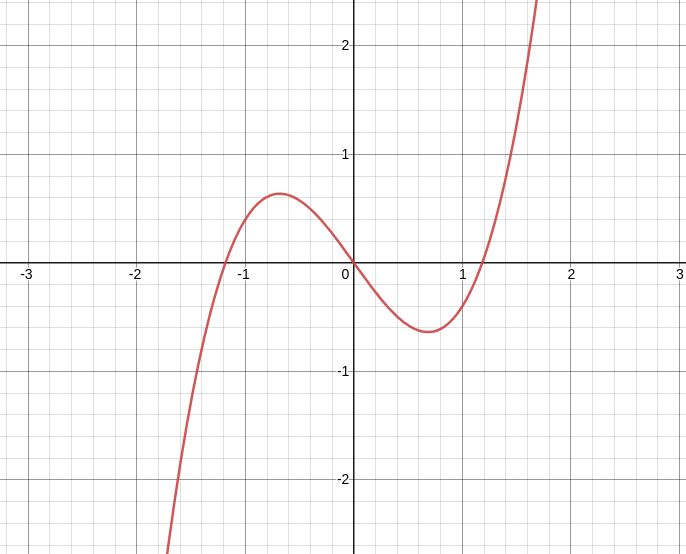
\includegraphics[scale=0.15]{figures/hP.png}
\caption{$x > 0$}
\label{fig:}
\end{subfigure}
\begin{subfigure}[b]{40mm}
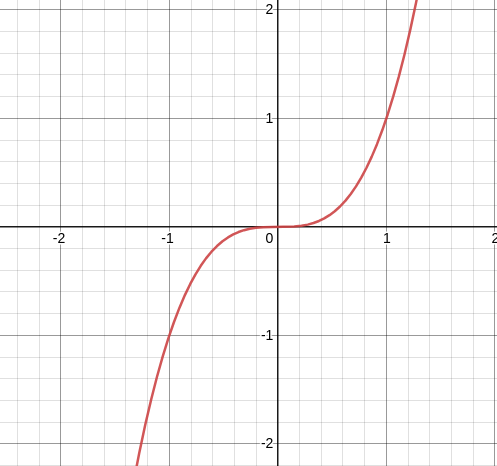
\includegraphics[scale=0.18]{figures/h0.png}
\caption{$x = 0$}
\label{fig:}
\end{subfigure}
\begin{subfigure}[b]{40mm}
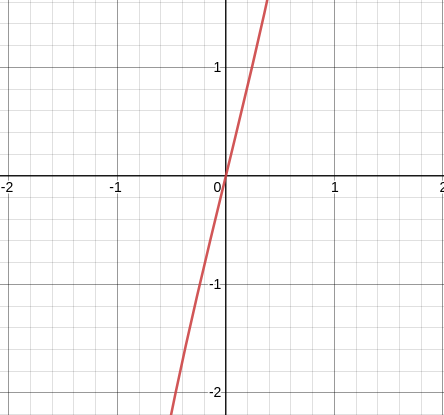
\includegraphics[scale=0.2]{figures/hN.png}
\caption{$x < 0$}
\label{fig:}
\end{subfigure}

\caption{The possible configurations of h}
\label{fig:}
\end{figure}
We find the stationary points of $h(z)$ to be $\pm\sqrt{\frac{x}{3}}$. We find $h^{\prime\prime}(z) = 6z -1$. Then 
\begin{align*}
u(x,t)\rightarrow \left[\frac{2\pi}{|6(\pm \sqrt{\frac{x}{3}} - 1)| \tau} \right]^{\frac{1}{2}} \left[ \frac{A}{2\pi} \frac{\sin\left( \frac{\tau \left(\pm \sqrt{\frac{x}{3}}\right)}{2} \right)}{\tau\left(\pm\sqrt{\frac{x}{3}}\right)} \right ] \exp\left\{i\tau\left(\left(\pm\sqrt{\frac{x}{3}}\right)^3 - \pm\sqrt{\frac{x}{3}}x \right)+ i\frac{\pi}{4}sign\left(6\left(\pm\sqrt{\frac{x}{3}}\right)\right)\right\}
\end{align*}
\section{Simulation results}
\begin{figure}[H]
\centering
\begin{subfigure}[b]{60mm}
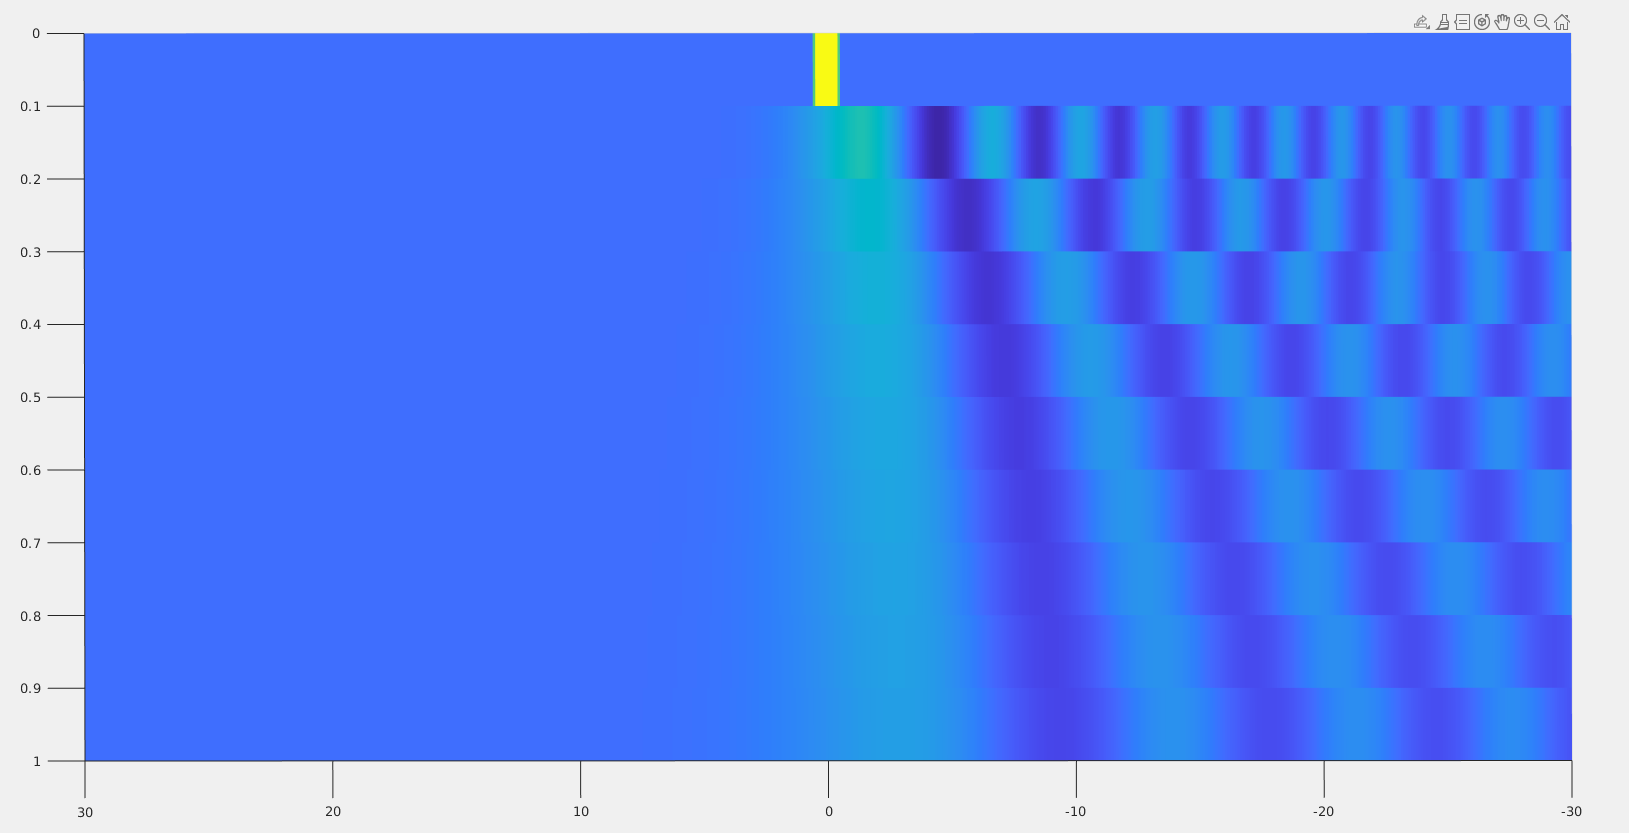
\includegraphics[scale=0.1]{figures/infl0p5H.png}
\caption{A = 0.5}
\label{fig:}
\end{subfigure}
\begin{subfigure}[b]{60mm}
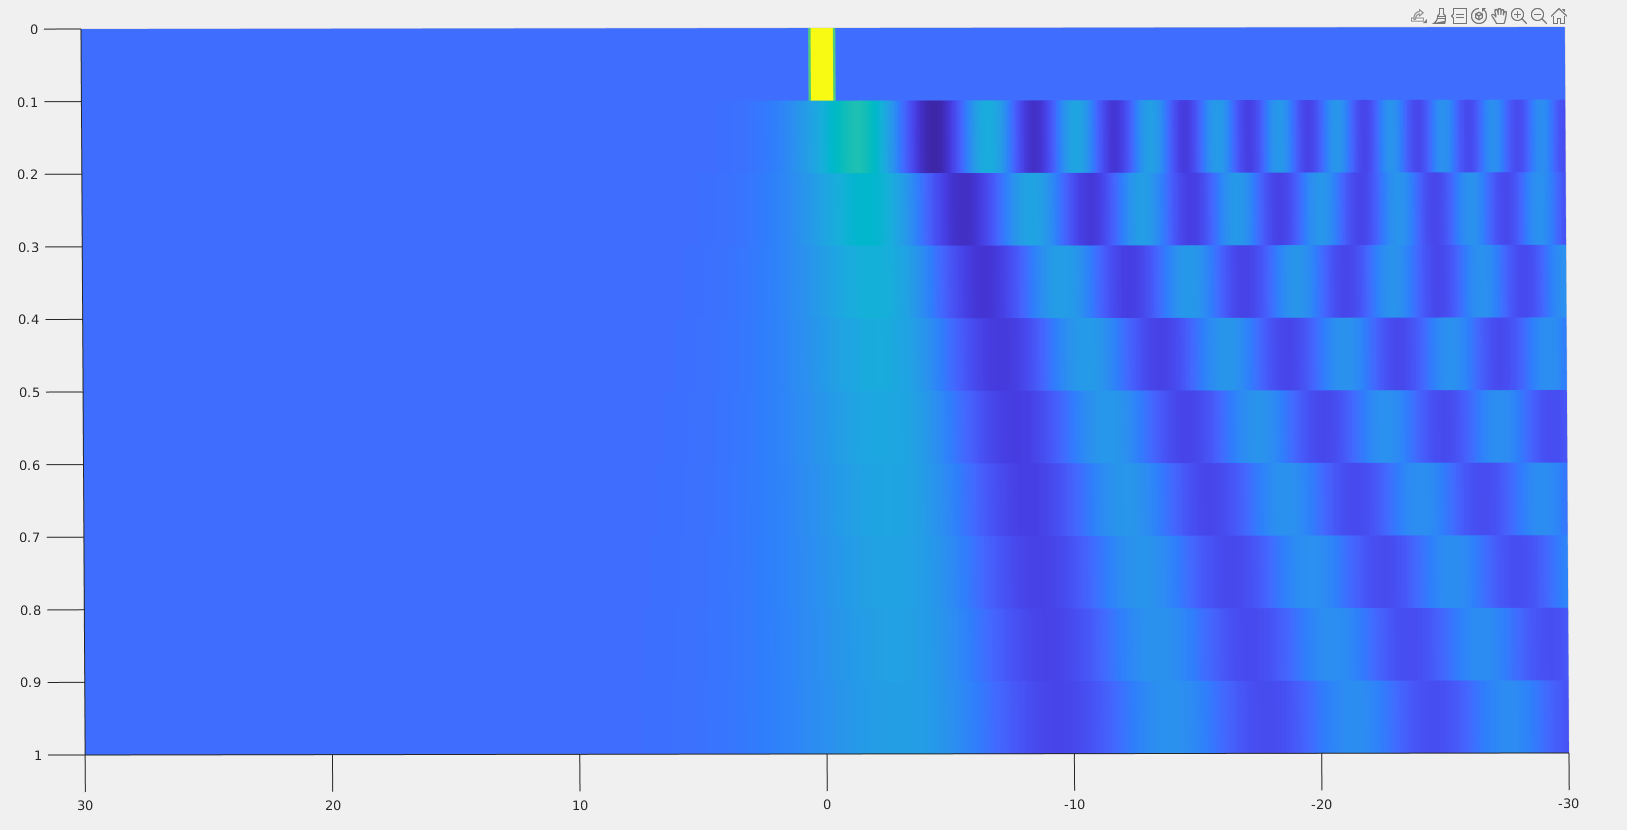
\includegraphics[scale=0.1]{figures/infl1H.png}
\caption{A = 1}
\label{fig:}
\end{subfigure}
\begin{subfigure}[b]{60mm}
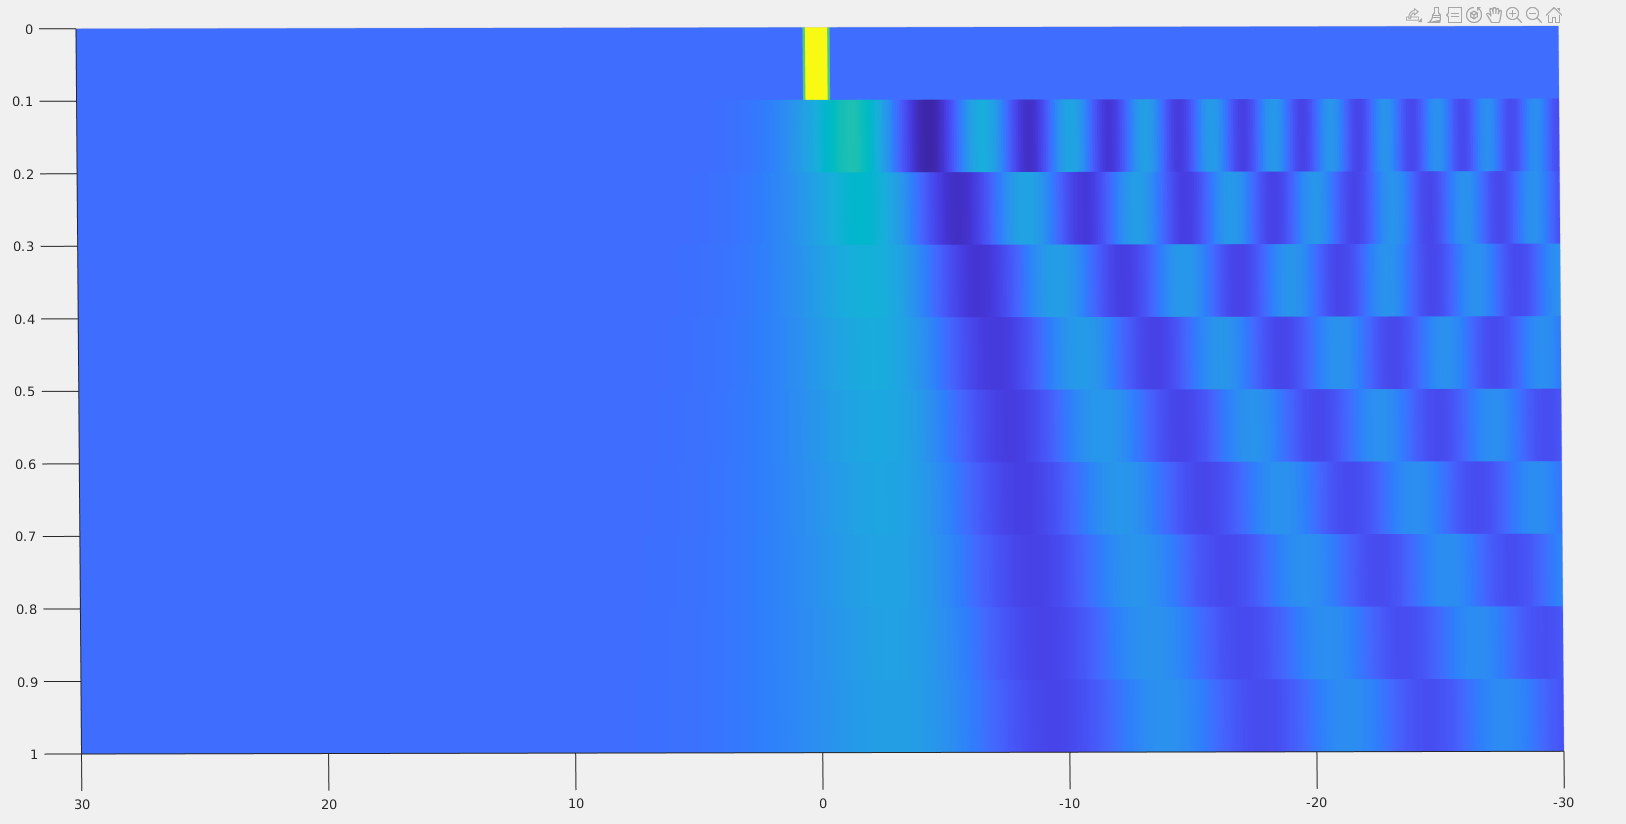
\includegraphics[scale=0.1]{figures/infl1p5H.png}
\caption{A = 1.5}
\label{fig:}
\end{subfigure}
\begin{subfigure}[b]{60mm}
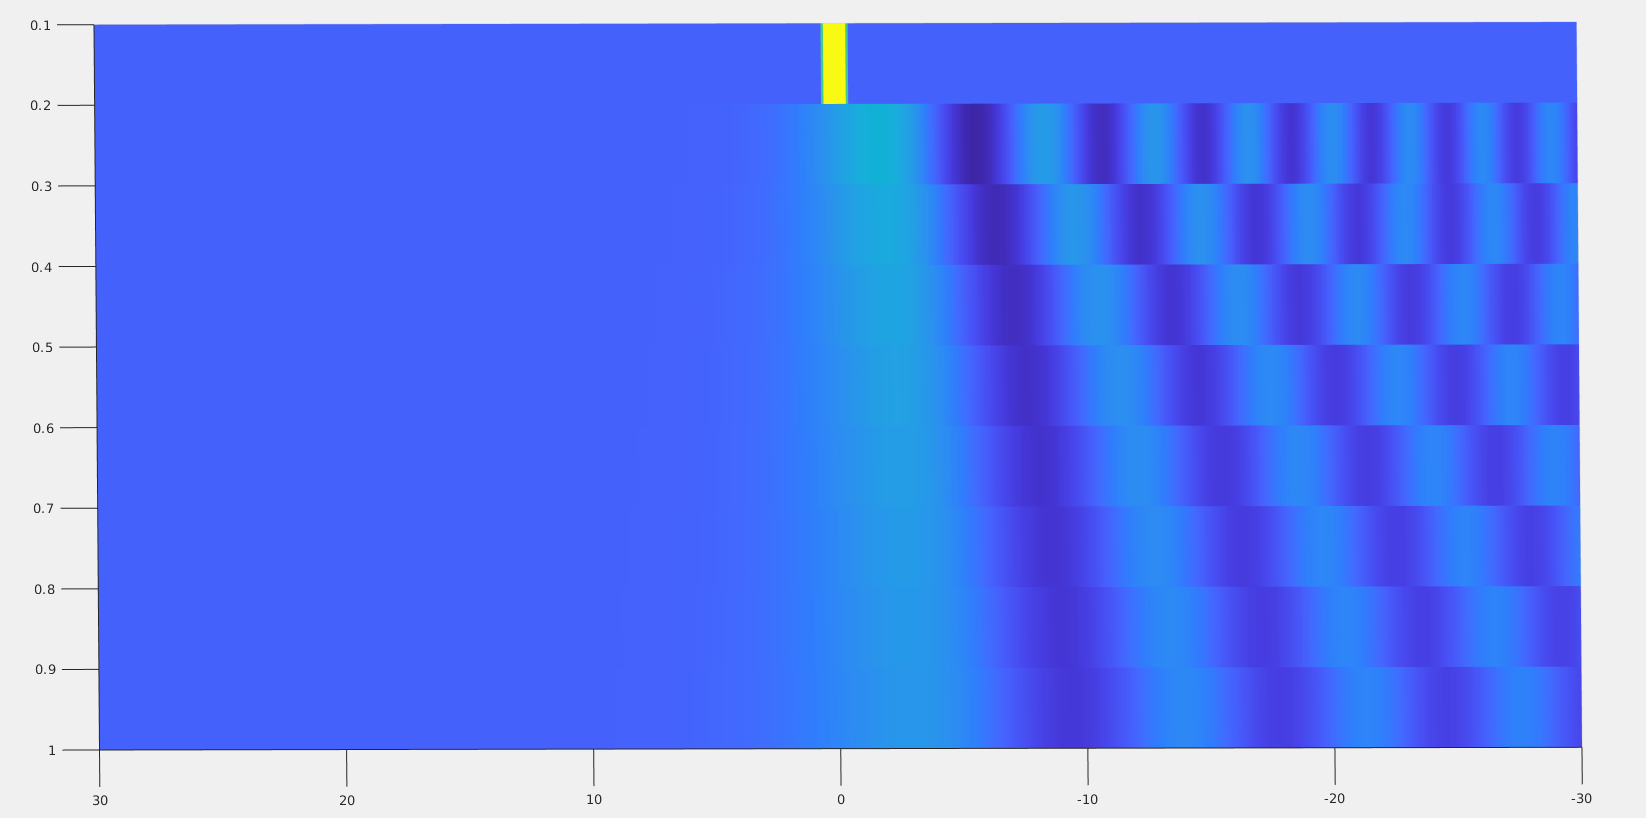
\includegraphics[scale=0.1]{figures/infl2H.png}
\caption{A = 2}
\label{fig:}
\end{subfigure}

\caption{Heat map of the influence function solution.}
\label{fig:}
\end{figure}

\begin{figure}[H]
\centering
\begin{subfigure}[b]{60mm}
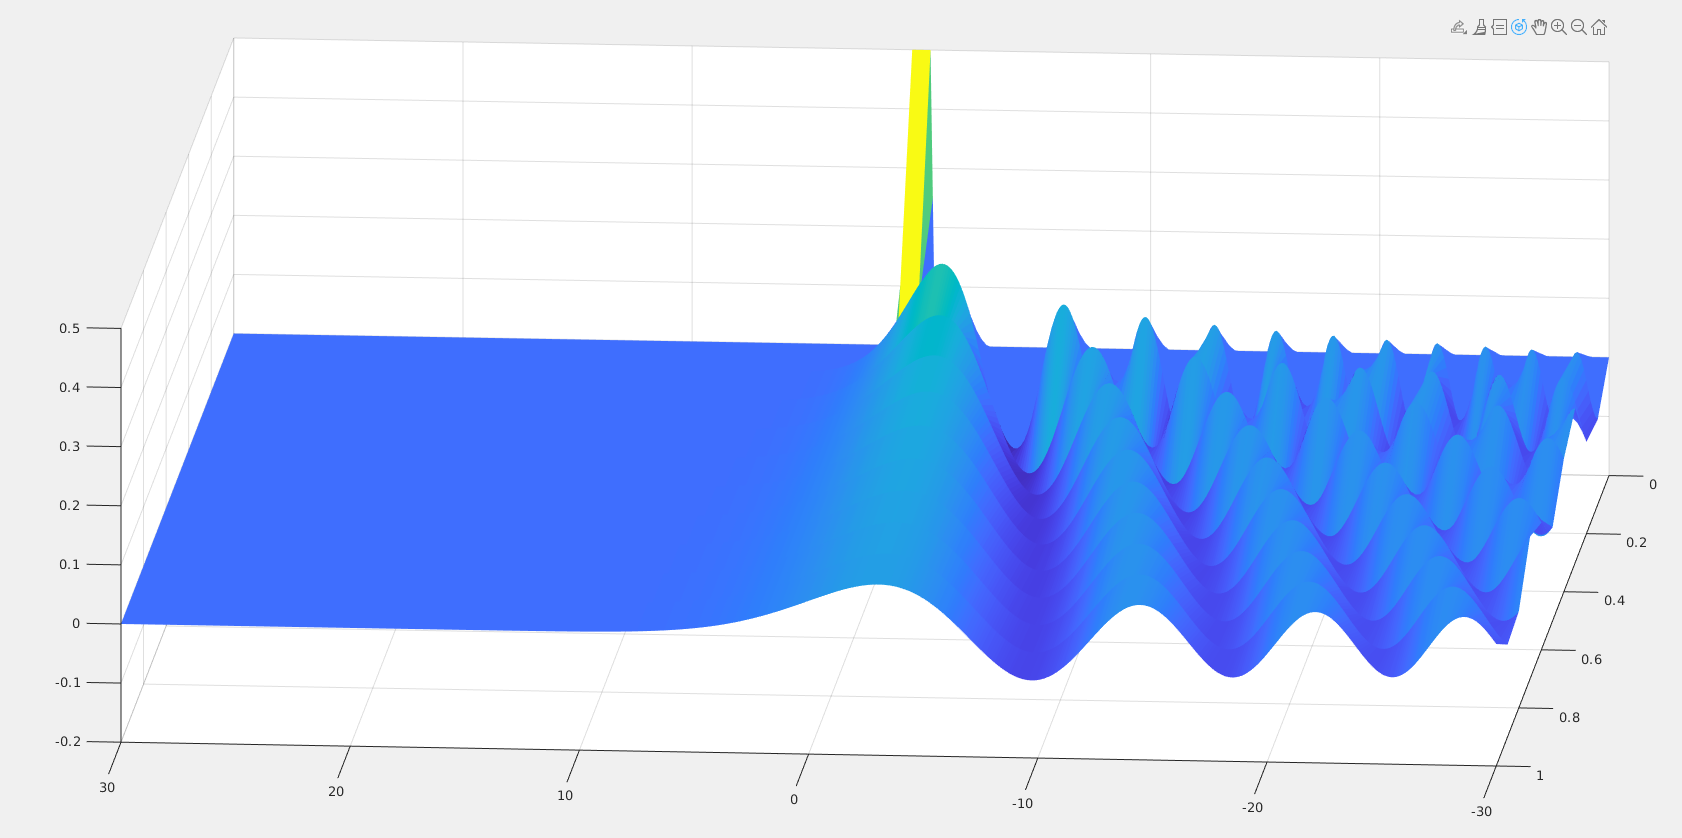
\includegraphics[scale=0.1]{figures/infl0p5V.png}
\caption{A = 0.5}
\label{fig:}
\end{subfigure}
\begin{subfigure}[b]{60mm}
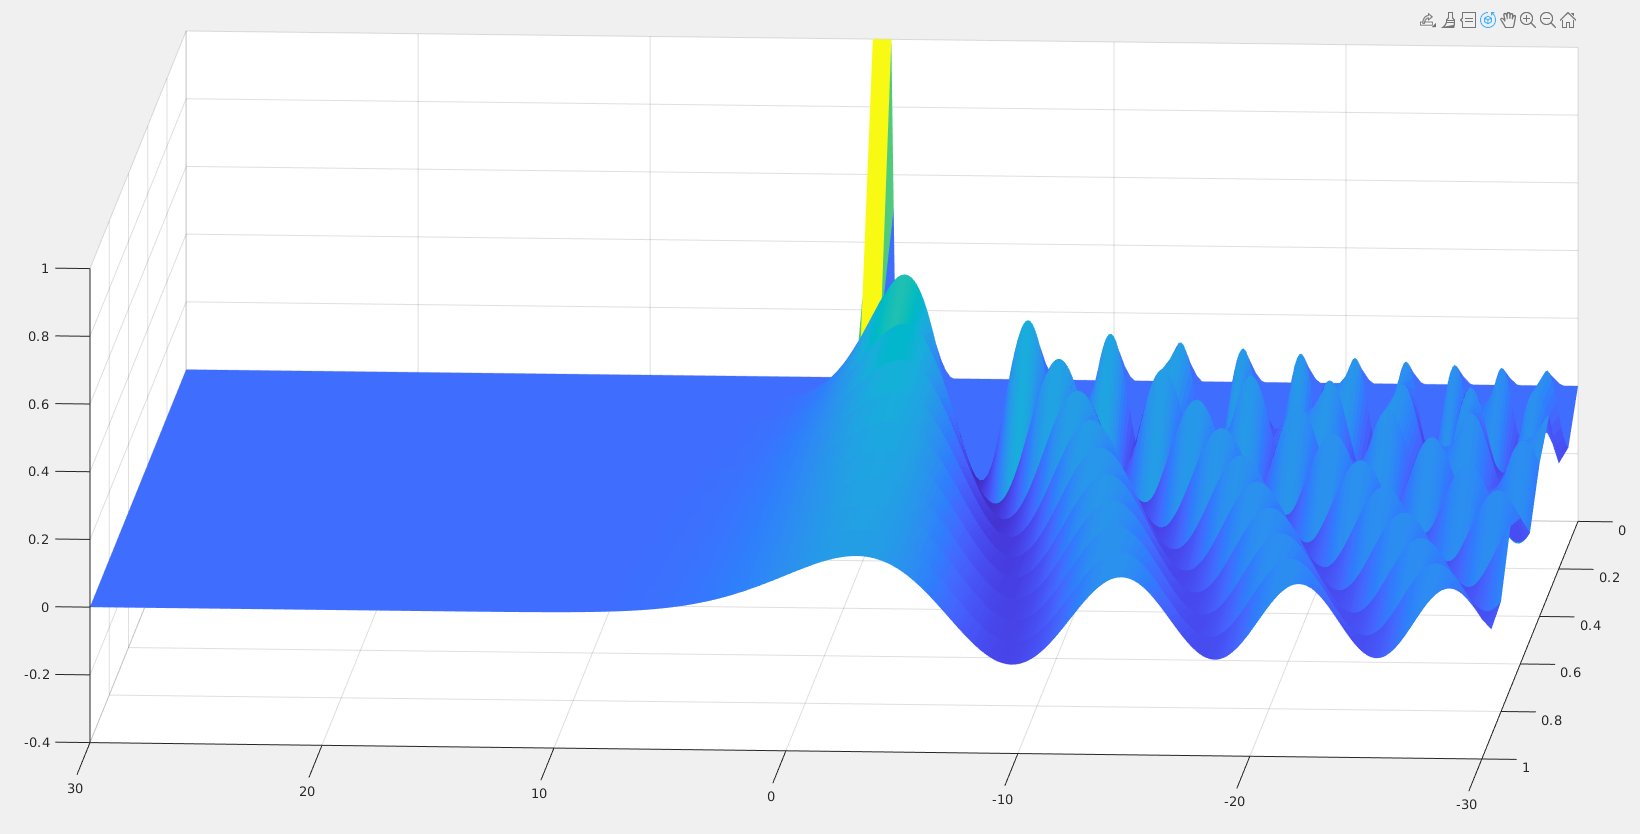
\includegraphics[scale=0.1]{figures/infl1V.png}
\caption{A = 1}
\label{fig:}
\end{subfigure}
\begin{subfigure}[b]{60mm}
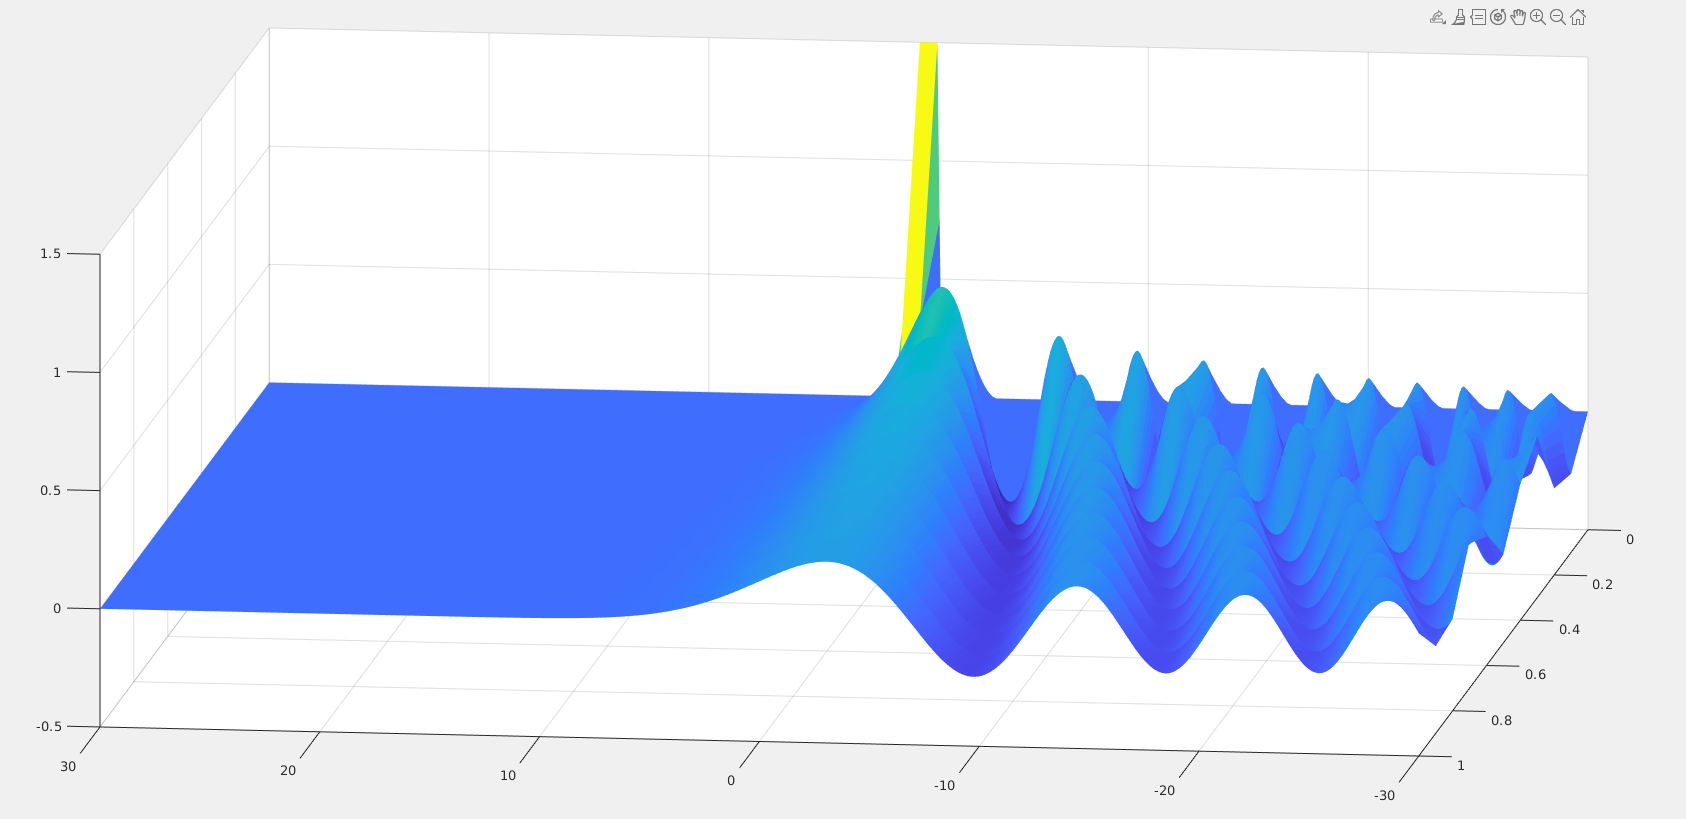
\includegraphics[scale=0.1]{figures/infl1p5V.png}
\caption{A = 1.5}
\label{fig:}
\end{subfigure}
\begin{subfigure}[b]{60mm}
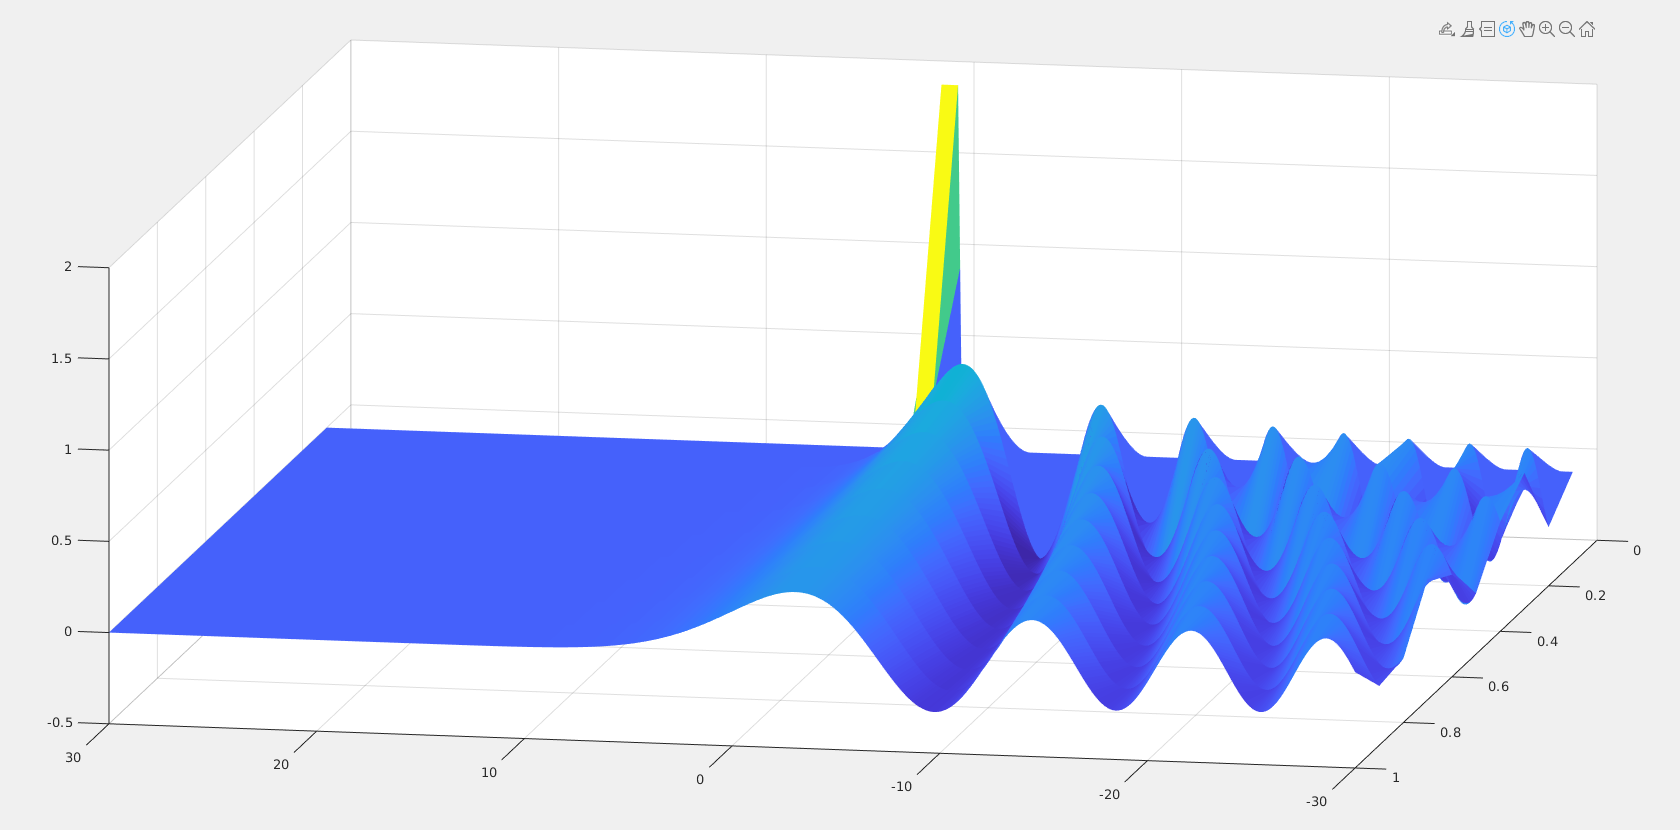
\includegraphics[scale=0.1]{figures/infl2V.png}
\caption{A = 2}
\label{fig:}
\end{subfigure}

\caption{Surface plot of the influence function solution.}
\label{fig:}
\end{figure}
\section{Numerical and analytical comparison}

\section{final remarks and conclusions}


\end{document}